\documentclass[12pt]{article}
%Fall 2022
% Some basic packages
\usepackage{standalone}[subpreambles=true]
\usepackage[utf8]{inputenc}
\usepackage[T1]{fontenc}
\usepackage{textcomp}
\usepackage[english]{babel}
\usepackage{url}
\usepackage{graphicx}
%\usepackage{quiver}
\usepackage{float}
\usepackage{enumitem}
\usepackage{lmodern}
\usepackage{comment}
\usepackage{hyperref}
\usepackage[usenames,svgnames,dvipsnames]{xcolor}
\usepackage[margin=1in]{geometry}
\usepackage{pdfpages}

\pdfminorversion=7

% Don't indent paragraphs, leave some space between them
\usepackage{parskip}

% Hide page number when page is empty
\usepackage{emptypage}
\usepackage{subcaption}
\usepackage{multicol}
\usepackage[b]{esvect}

% Math stuff
\usepackage{amsmath, amsfonts, mathtools, amsthm, amssymb}
\usepackage{bbm}
\usepackage{stmaryrd}
\allowdisplaybreaks

% Fancy script capitals
\usepackage{mathrsfs}
\usepackage{cancel}
% Bold math
\usepackage{bm}
% Some shortcuts
\newcommand{\rr}{\ensuremath{\mathbb{R}}}
\newcommand{\zz}{\ensuremath{\mathbb{Z}}}
\newcommand{\qq}{\ensuremath{\mathbb{Q}}}
\newcommand{\nn}{\ensuremath{\mathbb{N}}}
\newcommand{\ff}{\ensuremath{\mathbb{F}}}
\newcommand{\cc}{\ensuremath{\mathbb{C}}}
\newcommand{\ee}{\ensuremath{\mathbb{E}}}
\newcommand{\hh}{\ensuremath{\mathbb{H}}}
\renewcommand\O{\ensuremath{\emptyset}}
\newcommand{\norm}[1]{{\left\lVert{#1}\right\rVert}}
\newcommand{\dbracket}[1]{{\left\llbracket{#1}\right\rrbracket}}
\newcommand{\ve}[1]{{\bm{#1}}}
\newcommand\allbold[1]{{\boldmath\textbf{#1}}}
\DeclareMathOperator{\lcm}{lcm}
\DeclareMathOperator{\im}{im}
\DeclareMathOperator{\coim}{coim}
\DeclareMathOperator{\dom}{dom}
\DeclareMathOperator{\tr}{tr}
\DeclareMathOperator{\rank}{rank}
\DeclareMathOperator*{\var}{Var}
\DeclareMathOperator*{\ev}{E}
\DeclareMathOperator{\dg}{deg}
\DeclareMathOperator{\aff}{aff}
\DeclareMathOperator{\conv}{conv}
\DeclareMathOperator{\inte}{int}
\DeclareMathOperator*{\argmin}{argmin}
\DeclareMathOperator*{\argmax}{argmax}
\DeclareMathOperator{\graph}{graph}
\DeclareMathOperator{\sgn}{sgn}
\DeclareMathOperator*{\Rep}{Rep}
\DeclareMathOperator{\Proj}{Proj}
\DeclareMathOperator{\mat}{mat}
\DeclareMathOperator{\diag}{diag}
\DeclareMathOperator{\aut}{Aut}
\DeclareMathOperator{\gal}{Gal}
\DeclareMathOperator{\inn}{Inn}
\DeclareMathOperator{\edm}{End}
\DeclareMathOperator{\Hom}{Hom}
\DeclareMathOperator{\ext}{Ext}
\DeclareMathOperator{\tor}{Tor}
\DeclareMathOperator{\Span}{Span}
\DeclareMathOperator{\Stab}{Stab}
\DeclareMathOperator{\cont}{cont}
\DeclareMathOperator{\Ann}{Ann}
\DeclareMathOperator{\Div}{div}
\DeclareMathOperator{\curl}{curl}
\DeclareMathOperator{\nat}{Nat}
\DeclareMathOperator{\gr}{Gr}
\DeclareMathOperator{\vect}{Vect}
\DeclareMathOperator{\id}{id}
\DeclareMathOperator{\Mod}{Mod}
\DeclareMathOperator{\sign}{sign}
\DeclareMathOperator{\Surf}{Surf}
\DeclareMathOperator{\fcone}{fcone}
\DeclareMathOperator{\Rot}{Rot}
\DeclareMathOperator{\grad}{grad}
\DeclareMathOperator{\atan2}{atan2}
\DeclareMathOperator{\Ric}{Ric}
\let\vec\relax
\DeclareMathOperator{\vec}{vec}
\let\Re\relax
\DeclareMathOperator{\Re}{Re}
\let\Im\relax
\DeclareMathOperator{\Im}{Im}
% Put x \to \infty below \lim
\let\svlim\lim\def\lim{\svlim\limits}

%wide hat
\usepackage{scalerel,stackengine}
\stackMath
\newcommand*\wh[1]{%
\savestack{\tmpbox}{\stretchto{%
  \scaleto{%
    \scalerel*[\widthof{\ensuremath{#1}}]{\kern-.6pt\bigwedge\kern-.6pt}%
    {\rule[-\textheight/2]{1ex}{\textheight}}%WIDTH-LIMITED BIG WEDGE
  }{\textheight}% 
}{0.5ex}}%
\stackon[1pt]{#1}{\tmpbox}%
}
\parskip 1ex

%Make implies and impliedby shorter
\let\implies\Rightarrow
\let\impliedby\Leftarrow
\let\iff\Leftrightarrow
\let\epsilon\varepsilon

% Add \contra symbol to denote contradiction
\usepackage{stmaryrd} % for \lightning
\newcommand\contra{\scalebox{1.5}{$\lightning$}}

% \let\phi\varphi

% Command for short corrections
% Usage: 1+1=\correct{3}{2}

\definecolor{correct}{HTML}{009900}
\newcommand\correct[2]{\ensuremath{\:}{\color{red}{#1}}\ensuremath{\to }{\color{correct}{#2}}\ensuremath{\:}}
\newcommand\green[1]{{\color{correct}{#1}}}

% horizontal rule
\newcommand\hr{
    \noindent\rule[0.5ex]{\linewidth}{0.5pt}
}

% hide parts
\newcommand\hide[1]{}

% si unitx
\usepackage{siunitx}
\sisetup{locale = FR}

%allows pmatrix to stretch
\makeatletter
\renewcommand*\env@matrix[1][\arraystretch]{%
  \edef\arraystretch{#1}%
  \hskip -\arraycolsep
  \let\@ifnextchar\new@ifnextchar
  \array{*\c@MaxMatrixCols c}}
\makeatother

\renewcommand{\arraystretch}{0.8}

\renewcommand{\baselinestretch}{1.5}

\usepackage{graphics}
\usepackage{epstopdf}

\RequirePackage{hyperref}
%%
%% Add support for color in order to color the hyperlinks.
%% 
\hypersetup{
  colorlinks = true,
  urlcolor = blue,
  citecolor = blue
}
%%fakesection Links
\hypersetup{
    colorlinks,
    linkcolor={red!50!black},
    citecolor={green!50!black},
    urlcolor={blue!80!black}
}
%customization of cleveref
\RequirePackage[capitalize,nameinlink]{cleveref}[0.19]

% Per SIAM Style Manual, "section" should be lowercase
\crefname{section}{section}{sections}
\crefname{subsection}{subsection}{subsections}
\Crefname{section}{Section}{Sections}
\Crefname{subsection}{Subsection}{Subsections}

% Per SIAM Style Manual, "Figure" should be spelled out in references
\Crefname{figure}{Figure}{Figures}

% Per SIAM Style Manual, don't say equation in front on an equation.
\crefformat{equation}{\textup{#2(#1)#3}}
\crefrangeformat{equation}{\textup{#3(#1)#4--#5(#2)#6}}
\crefmultiformat{equation}{\textup{#2(#1)#3}}{ and \textup{#2(#1)#3}}
{, \textup{#2(#1)#3}}{, and \textup{#2(#1)#3}}
\crefrangemultiformat{equation}{\textup{#3(#1)#4--#5(#2)#6}}%
{ and \textup{#3(#1)#4--#5(#2)#6}}{, \textup{#3(#1)#4--#5(#2)#6}}{, and \textup{#3(#1)#4--#5(#2)#6}}

% But spell it out at the beginning of a sentence.
\Crefformat{equation}{#2Equation~\textup{(#1)}#3}
\Crefrangeformat{equation}{Equations~\textup{#3(#1)#4--#5(#2)#6}}
\Crefmultiformat{equation}{Equations~\textup{#2(#1)#3}}{ and \textup{#2(#1)#3}}
{, \textup{#2(#1)#3}}{, and \textup{#2(#1)#3}}
\Crefrangemultiformat{equation}{Equations~\textup{#3(#1)#4--#5(#2)#6}}%
{ and \textup{#3(#1)#4--#5(#2)#6}}{, \textup{#3(#1)#4--#5(#2)#6}}{, and \textup{#3(#1)#4--#5(#2)#6}}

% Make number non-italic in any environment.
\crefdefaultlabelformat{#2\textup{#1}#3}

% Environments
\makeatother
% For box around Definition, Theorem, \ldots
%%fakesection Theorems
\usepackage{thmtools}
\usepackage[framemethod=TikZ]{mdframed}

\theoremstyle{definition}
\mdfdefinestyle{mdbluebox}{%
	roundcorner = 10pt,
	linewidth=1pt,
	skipabove=12pt,
	innerbottommargin=9pt,
	skipbelow=2pt,
	nobreak=true,
	linecolor=blue,
	backgroundcolor=TealBlue!5,
}
\declaretheoremstyle[
	headfont=\sffamily\bfseries\color{MidnightBlue},
	mdframed={style=mdbluebox},
	headpunct={\\[3pt]},
	postheadspace={0pt}
]{thmbluebox}

\mdfdefinestyle{mdredbox}{%
	linewidth=0.5pt,
	skipabove=12pt,
	frametitleaboveskip=5pt,
	frametitlebelowskip=0pt,
	skipbelow=2pt,
	frametitlefont=\bfseries,
	innertopmargin=4pt,
	innerbottommargin=8pt,
	nobreak=false,
	linecolor=RawSienna,
	backgroundcolor=Salmon!5,
}
\declaretheoremstyle[
	headfont=\bfseries\color{RawSienna},
	mdframed={style=mdredbox},
	headpunct={\\[3pt]},
	postheadspace={0pt},
]{thmredbox}

\declaretheorem[%
style=thmbluebox,name=Theorem,numberwithin=section]{thm}
\declaretheorem[style=thmbluebox,name=Lemma,sibling=thm]{lem}
\declaretheorem[style=thmbluebox,name=Proposition,sibling=thm]{prop}
\declaretheorem[style=thmbluebox,name=Corollary,sibling=thm]{coro}
\declaretheorem[style=thmredbox,name=Example,sibling=thm]{eg}

\mdfdefinestyle{mdgreenbox}{%
	roundcorner = 10pt,
	linewidth=1pt,
	skipabove=12pt,
	innerbottommargin=9pt,
	skipbelow=2pt,
	nobreak=true,
	linecolor=ForestGreen,
	backgroundcolor=ForestGreen!5,
}

\declaretheoremstyle[
	headfont=\bfseries\sffamily\color{ForestGreen!70!black},
	bodyfont=\normalfont,
	spaceabove=2pt,
	spacebelow=1pt,
	mdframed={style=mdgreenbox},
	headpunct={ --- },
]{thmgreenbox}

\declaretheorem[style=thmgreenbox,name=Definition,sibling=thm]{defn}

\mdfdefinestyle{mdgreenboxsq}{%
	linewidth=1pt,
	skipabove=12pt,
	innerbottommargin=9pt,
	skipbelow=2pt,
	nobreak=true,
	linecolor=ForestGreen,
	backgroundcolor=ForestGreen!5,
}
\declaretheoremstyle[
	headfont=\bfseries\sffamily\color{ForestGreen!70!black},
	bodyfont=\normalfont,
	spaceabove=2pt,
	spacebelow=1pt,
	mdframed={style=mdgreenboxsq},
	headpunct={},
]{thmgreenboxsq}
\declaretheoremstyle[
	headfont=\bfseries\sffamily\color{ForestGreen!70!black},
	bodyfont=\normalfont,
	spaceabove=2pt,
	spacebelow=1pt,
	mdframed={style=mdgreenboxsq},
	headpunct={},
]{thmgreenboxsq*}

\mdfdefinestyle{mdblackbox}{%
	skipabove=8pt,
	linewidth=3pt,
	rightline=false,
	leftline=true,
	topline=false,
	bottomline=false,
	linecolor=black,
	backgroundcolor=RedViolet!5!gray!5,
}
\declaretheoremstyle[
	headfont=\bfseries,
	bodyfont=\normalfont\small,
	spaceabove=0pt,
	spacebelow=0pt,
	mdframed={style=mdblackbox}
]{thmblackbox}

\theoremstyle{plain}
\declaretheorem[name=Question,sibling=thm,style=thmblackbox]{ques}
\declaretheorem[name=Remark,sibling=thm,style=thmgreenboxsq]{remark}
\declaretheorem[name=Remark,sibling=thm,style=thmgreenboxsq*]{remark*}
\newtheorem{ass}[thm]{Assumptions}

\theoremstyle{definition}
\newtheorem*{problem}{Problem}
\newtheorem{claim}[thm]{Claim}
\theoremstyle{remark}
\newtheorem*{case}{Case}
\newtheorem*{notation}{Notation}
\newtheorem*{note}{Note}
\newtheorem*{motivation}{Motivation}
\newtheorem*{intuition}{Intuition}
\newtheorem*{conjecture}{Conjecture}

% Make section starts with 1 for report type
%\renewcommand\thesection{\arabic{section}}

% End example and intermezzo environments with a small diamond (just like proof
% environments end with a small square)
\usepackage{etoolbox}
\AtEndEnvironment{vb}{\null\hfill$\diamond$}%
\AtEndEnvironment{intermezzo}{\null\hfill$\diamond$}%
% \AtEndEnvironment{opmerking}{\null\hfill$\diamond$}%

% Fix some spacing
% http://tex.stackexchange.com/questions/22119/how-can-i-change-the-spacing-before-theorems-with-amsthm
\makeatletter
\def\thm@space@setup{%
  \thm@preskip=\parskip \thm@postskip=0pt
}

% Fix some stuff
% %http://tex.stackexchange.com/questions/76273/multiple-pdfs-with-page-group-included-in-a-single-page-warning
\pdfsuppresswarningpagegroup=1


% My name
\author{Jaden Wang}



\begin{document}
\centerline {\textsf{\textbf{\LARGE{Homework 1}}}}
\centerline {Jaden Wang}
\vspace{.15in}
\begin{problem}[1]
\begin{enumerate}[label=(\alph*)]
	\item $ \mathcal{ D}$ is not closed and therefore not compact as it is missing the limit point $ 4 \pi$. Weierstrass theorem only applies to compact sets. The infimum of $ f( \mathcal{ D})$ is achieved as minimum by $ f\left( \frac{3}{2} \pi \right) = -1$. $ \mathcal{ D}$ is convex as any type of interval contains all line segments between any two points. $ f$ is not convex since its epigraph (region above the sine wave) is clearly not a convex set (take two points in different ''vallys", and the line segment is not contained in the epigraph.) Global, strictly global, local, strictly local, and isolated local minimizers all coincide in this case. They are $-\frac{5}{2}\pi, -\frac{1}{2} \pi, \frac{3}{2}\pi, \frac{7}{2} \pi$.
	\item $ \mathcal{ D}$ is closed since $ \rr$ is clopen. But it is not compact as it is not bounded. Thus Weierstrass doesn't apply. The infimum is $1- \sup| \arctan x| = 1 - \frac{\pi}{ 2}$. The minimum doesn't exist, implying that minimizers also don't exist. $ \mathcal{ D}$ is convex but $ f$ is not as its epigraph is not.
	\item  $ \mathcal{ D}$ is not closed as it is missing the limit point 0. Thus it is not compact and Weierstrass doesn't apply. The infimum is achieved as minimum by $ f(4.49) = -0.22$.  $ \mathcal{ D}$ is an open interval and thus convex but $ f$ is not since it is still a wave and its epigraph is not convex.
	\item  $ \mathcal{ D}$ is closed because it contains all its limit points. It is also compact since it is bounded (or it clearly always admits a finite subcover). Thus Weierstrass applies. The infimum is achieved as minimum by $ f(0) = 0$.  $ \mathcal{ D}$ is clearly not convex so $ f$ is not convex as convex function requires the domain to be convex. Its global and strictly global minimizer is 0, and every nonzero point in the domain is a local, strictly local, and isolated local minimizer of  $ f$, whereas 0 is everything but an isolated local minimizer.
\end{enumerate}
\end{problem}

\begin{problem}[2]
\begin{enumerate}[label=(\alph*)]
	\item Converting to matrix form, we have
	\begin{align*}
		f(x,y) = \begin{pmatrix} x&y \end{pmatrix}  \begin{pmatrix} 1&1\\1&3 \end{pmatrix} \begin{pmatrix} x\\y \end{pmatrix}  + \begin{pmatrix} 2&10 \end{pmatrix}  \begin{pmatrix} x\\y \end{pmatrix} + 9
	\end{align*}
	Since $ A$ is positive definite, applying the quadratic minimization lemma yields 
\begin{align*}
	f^* &= c - \frac{1}{4}b^{T}A^{-1}b\\
	    &= 9 - \frac{1}{4} \begin{pmatrix} 2&10 \end{pmatrix} \frac{1}{2}\begin{pmatrix} 3&-1\\-1&1 \end{pmatrix} \begin{pmatrix} 2\\10 \end{pmatrix}  \\
	    &= 9-9=0 
\end{align*}
\item The matrix form is
	\begin{align*}
	f(x,y) = \begin{pmatrix} x&y \end{pmatrix}  \begin{pmatrix} 2&\frac{3}{2}\\\frac{3}{2}&0 \end{pmatrix} \begin{pmatrix} x\\y \end{pmatrix}  + \begin{pmatrix} -3&1 \end{pmatrix}  \begin{pmatrix} x\\y \end{pmatrix} -8
	\end{align*}
\end{enumerate}
Since $ A$ is not positive semidefinite, we cannot apply the quadratic minimization lemma.
 \begin{align*}
f^* &= c - \frac{1}{4}b^{T}A^{-1}b\\
	    &= -8 - \frac{1}{4} \begin{pmatrix} -3&1 \end{pmatrix} \frac{-4}{9}\begin{pmatrix} 0&-\frac{3}{2}\\-\frac{3}{2}&2 \end{pmatrix} \begin{pmatrix} -3\\1 \end{pmatrix}  \\
	    &=-8+\frac{11}{9} = - \frac{61}{9} 
\end{align*}

\end{problem}
\begin{problem}[3]
\begin{enumerate}[label=(\roman*)]
	\item A minimum hence infimum exists at $ f(0) = 0$. $ \mathcal{ D}$ is not closed or compact so we cannot apply Weierstrass.
	\item A minimum or even an infimum doesn't exist as $ f$ is not bounded from below in its domain. $ \mathcal{ D}$ is not closed nor compact so we cannot apply Weierstrass.
	\item  A minimum hence infimim exists at $ f(0) = 0$. $ f$ is not continuous so we cannot apply Weierstrass.
\end{enumerate}
\end{problem}

\begin{problem}[4]
\begin{enumerate}[label=(\roman*)]
	\item The feasible cone is itself: $ \{(x,y):y \geq 0\} $.
	\item The feasible cone is $ \{(x,y):x < 0\} \cup \{(0,0)\}$,
	\item The slope of the tangent line at $ x=3$ is 6. The feasible cone is $ \{(x,y): y > 6x\} \cup \{(0,0)\}  $.
\end{enumerate}
\end{problem}

\begin{problem}[5]
The feasible cone is $ \rr^2$ so
\begin{align*}
	D_+f((0,0);(\xi_1,\xi_2)) &= \lim_{ h \to 0^+} \frac{f(h\xi_1,h\xi_2) - f(0,0)}{ h} \\
	&=\lim_{ h \to 0^+} \frac{h \sqrt{\xi_1^2+\xi_2^2} }{ h}   \\
	&=\sqrt{ \xi_1^2+ \xi_2^2}  
\end{align*}
\end{problem}

\begin{problem}[6]
Some work such as partial fraction decomposition is done on scratch paper. Integrals are computed by Wolfram alpha.
\begin{enumerate}[label=(\arabic*)]
\item $ u(t) = t$. We first apply Laplace transform to solve for $ x(t)$ and then evaluate the integral:
 \begin{align*}
	\mathcal{L}\left\{ \dot{x}\right\}  &= \mathcal{L}\left\{ 2x\right\} + \mathcal{L}\left\{ t\right\}  \\
	sX(s) - x(0)&= 2X(s) + \frac{1}{s^2} \\
	X(s) &= -\frac{1}{4} \left( \frac{1}{s} \right) + \frac{2}{s^2} + \frac{1}{4} \frac{1}{s-2} + \frac{1}{s-2}\\
	\mathcal{L}^{-1}\left\{ X(s)\right\} &= \mathcal{L}^{-1}\left\{ -\frac{1}{4} \left( \frac{1}{s} \right) + \frac{2}{s^2} + \frac{1}{4} \frac{1}{s-2} + \frac{1}{s-2}\right\}  \\
	x(t) &= \frac{5}{4} e^{2t}-\frac{1}{2}t -\frac{1}{4} \\
	x(1) &= \frac{5}{4}e^2 - \frac{3}{4} \\
	J(t) &= (x(1)-3)^2 + \frac{1}{2} \int_{ 0}^{ 1}\left[    \left( \frac{5}{4} e^{2t}-\frac{1}{2}t -\frac{1}{4} \right)^2 + t^2 \right] dt  \\
	&= 38.56 
\end{align*}
\item $ u(t) = e^{t}$.
\begin{align*}
	\mathcal{L}\left\{ \dot{x}\right\} &= \mathcal{L}\left\{ 2x\right\} + \mathcal{L}\left\{ e^{t}\right\}  \\
	sX(s) - x(0)&= 2X(s) + \frac{1}{s-1} \\
	X(s)&= \frac{1}{s-2} + \frac{1}{(s-1)(s-2)} \\
	X(s) &= 2\frac{1}{s-2}-\frac{1}{s-1} \\
	\mathcal{L}^{-1}\left\{ X(s)\right\} &= 2\mathcal{L}^{-1}\left\{ \frac{1}{s-2}\right\} - \mathcal{L}^{-1}\left\{ \frac{1}{s-1}\right\}  \\
	x(t)&= 2e^{2t}- e^{t} \\
	x(1) &= 2e ^2 - e \\
	J(e^t) &= (x(1)-3)^2 + \frac{1}{2} \int_{ 0}^{ 1}\left[    \left( 2 e^{2t}-e^t \right)^2 + e^{2t} \right] dt  \\
	&= 99.35 \\
\end{align*}
\item $ u(t) = 2e^{-t}$.
\begin{align*}
	\mathcal{L}\left\{ \dot{x}\right\} &= \mathcal{L}\left\{ 2x\right\} + \mathcal{L}\left\{ 2e^{-t}\right\}  \\
	sX(s) - x(0)&= 2 X(s) + 2 \frac{1}{s+1} \\
	X(s) &= \frac{1}{s-2} + 2 \frac{1}{(s+1)(s-2)} \\
	X(s) &= \frac{5}{3} \frac{1}{s-2} - \frac{2}{3} \frac{1}{s+1} \\
	\mathcal{L}^{-1}\left\{ X(s)\right\} &=\frac{5}{3} \mathcal{L}^{-1}\left\{ \frac{1}{s-2}\right\} - \frac{2}{3} \mathcal{L}^{-1}\left\{ \frac{1}{s+1}\right\}  \\
	x(t)&= \frac{5}{3} e^{2t} - \frac{2}{3} e^{-t} \\
	x(1) &= \frac{5}{3} e ^2 - \frac{2}{3} e^{-1} \\ 
	J(2e^{-t}) &= (x(1)-3)^2 + \frac{1}{2} \int_{ 0}^{ 1}\left[    \left( \frac{5}{3} e^{2t}-\frac{2}{3}e^{-t} \right)^2 + 4e^{-2t} \right] dt  \\
	&= 99.92 
\end{align*}
\end{enumerate}
Thus, $ u_1$ gives the smallest value.
\end{problem}

\begin{problem}[7]
Since $ f$ is 
 \begin{align*}
	 Df(x,y) &= \begin{pmatrix} 2x-2&2\\y&x+2y \end{pmatrix}  \\
	 Df((2,2);(1,-1))&= Df(2,2) \begin{pmatrix} 1\\-1 \end{pmatrix}  \\
			 &= \begin{pmatrix} 2&2\\2&6 \end{pmatrix} \begin{pmatrix} 1\\-1 \end{pmatrix}  \\
			 &= \begin{pmatrix} 0\\-4 \end{pmatrix}  
\end{align*}
\end{problem}

\begin{problem}[8]
Choose $ \epsilon = \frac{1}{2}$. For any $ \delta > 0$, choose $ x_2= x_1^2$ s.t.\ $ x_1^2+x_2^2\leq \delta^2$. Since $ f(0,0)=0$, we have
\begin{align*}
	|f(x_1,x_2) - 0| = |f(x_1,x_2)| = 1 \geq \frac{1}{2}.
\end{align*}
Hence $ f$ is discontinuous at  $ (0,0)$.

The feasible cone at $ (0,0)$ is  $ \rr^2$. Notice if $ t x_2 = t^2 x_1^2, t\neq 0 \implies x_2 = t x_1^2$, then such value of $ t$ is unique except when  $ x_1=x_2=0$. Thus if we take $ (x_1,x_2) \neq (0,0)$, $ t x_2 \neq t^2 x_1^2 \ \forall \ t \neq 0$ except for that unique value, so
\begin{align*}
	Df((0,0);(x_1,x_2))&= \lim_{ t \to 0}  \frac{f(tx_1,tx_2)-f(0,0)}{ t} \\
	&= \lim_{ t \to 0} \frac{0-0}{ t} =0
\end{align*}
Thus $ f$ is G\^{a}teaux differentiable.
\end{problem}

\begin{problem}[9]
\begin{enumerate}[label=(\alph*)]
	\item Explicitly, $ g(a) = (ah_2-pa^2h_1^2)(ah_2-qa^2h_1^2)$ and $ g'(a) = (h_2-2ph_1^2a)(h_2a-qh_1^2a^2)+(h_2a-ph_1^2a^2)(h_2-2qh_1^2a)$. Since the feasible cone at $ (0,0)$ is  $ \rr^2$,
	\begin{align*}
		g'(0)=Df((0,0);(h_1,h_2)) &= \lim_{ a \to 0} \frac{g(a)-g(0)}{ a} \\
		&= \lim_{ a \to 0} \frac{(ah_2-pa^2h_1^2)(ah_2-qa^2h_1^2)-0}{ a} \\
		&=0  \\
		g''(0) = D^2f((0,0);(h_1,h_2)) &= \lim_{ a \to 0} \frac{g'(a)-g'(0)}{ a} \\
		&= \lim_{ a \to 0} (h_2-2ph_1^2 a)(h_2-qh_1^2a) + (h_2-ph_1^2a)(h_2-2qh_1^2 a) \\
		&= 2h_2^2  \geq 0
	\end{align*}
	Therefore, by the sufficient conditions of local minimizer, $ a=0$ is a local minimizer of  $ g$, as desired.
\item 
	\begin{align*}
		Df(y,z)&= \begin{pmatrix} -2py(z-qy^2)-2qy(z-py^2)& 2z-(p+q)y^2 \end{pmatrix}  \\
		Df(x_0) &= 0 
	\end{align*}
\item $ f(x_0) = 0$. It suffices to find an $ x$  s.t.\ $ f(x)<0$. We just need the two factors to have different signs. Fix an $ y\neq 0$, choose  $ z$  s.t.\ $ py^2<z<qy^2$ which is possible since $ p<q$. Then clearly the two factors have different signs so $ f(y,z)<0$.
\item 
~\begin{figure}[H]
	\centering
	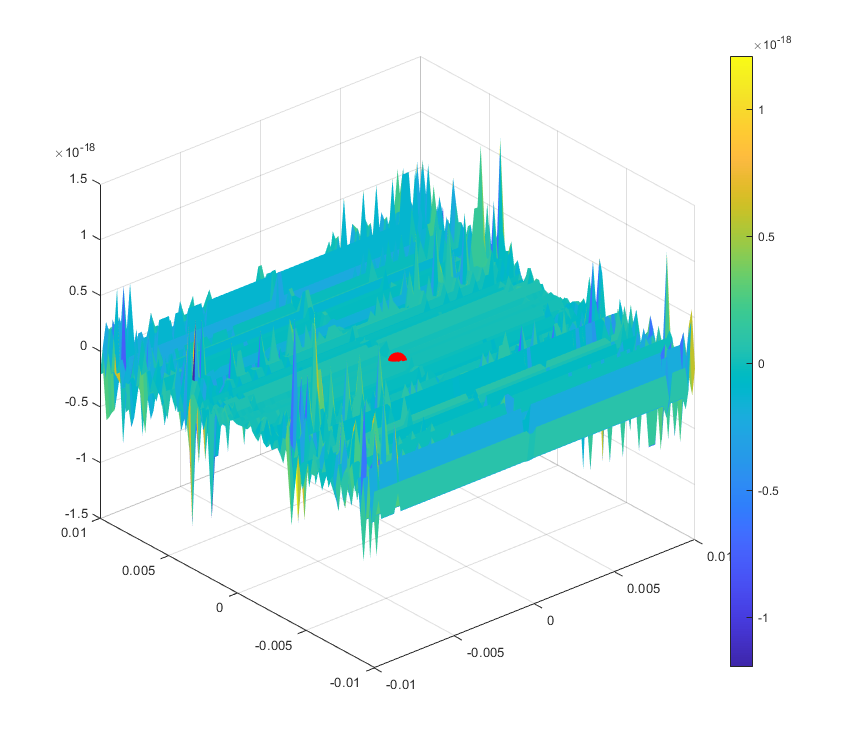
\includegraphics[width=0.8\textwidth]{./figures/hw01_plot.png}
	\caption{The red dot is (0,0). The function behaves erratically near the origin so there is no neighborhood where it can be a local minimizer.}
\end{figure}
\end{enumerate}
\end{problem}
\end{document}
